\clearpage{\pagestyle{empty}\cleardoublepage}
\chapter{Caratteristiche della memoria cache}

%\begin{flushright}\begin{small}\textit{"The beginning of knowledge\\
% is the discovery of something we do not understand."}\\
%- Frank Herbert -\\
%\end{small}\end{flushright}

La cache progettata \`e di tipo Set-Associative: [spiegare cosa significa].


Per garantire maggiore flessibilit\`a si \`e scelto di parametrizzare alcune delle caratteristiche statiche della cache, quali ad esempio:
\begin{itemize}
\item la dimensione dei blocchi
\item	il numero di vie 
\item il numero di linee
\end{itemize}


L'algoritmo di rimpiazzamento \`e basato su contatori.


\subsubsection{Struttura e interfacce}
La memoria cache si interfaccia con i dispositivi esterni attraverso 3 tipi di interfacce, come mostrato in \ref{fig:int_gen}.

\begin{figure}[!h]
 \centering
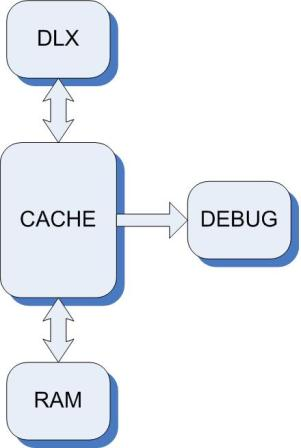
\includegraphics{img/01-interfacce_schema_generale.jpg}
 \caption{Interfacce della memoria cache}
 \label{fig:int_gen}
\end{figure}
